\documentclass[a4paper,11pt]{article}
\usepackage[T1]{fontenc}
\usepackage[utf8]{inputenc}
\renewcommand{\figurename}{Slika}\renewcommand{\refname}{Viri}
\usepackage{graphicx}
\usepackage{float}
\usepackage[margin=2.5cm]{geometry}
\usepackage{hyperref}

\title{Pregled obstoječih rešitev\\[4pt]\large Projekt za podjetje Dewesoft}
\author{Nejc Toplak, Leon, Bedenik\\[4pt]
Interaktivne tehnologije in komunikacija (ITK VS), FERI Maribor}
\date{23.~november 2026}

\begin{document}
\maketitle

\section{Uvod}
Podjetje Dewesoft razvija opremo in programsko opremo za zajem podatkov (DAQ), uporabniki pa so predvsem inženirji in študenti. Stranka mora danes za izbiro opreme, prenos programa, iskanje odgovorov in učenje uporabljati več delov spletišča: Academy, podporni portal, forum, razvijalski portal in prenose~\cite{dws-signin}.

Naš projekt je enoten spletni portal za stranke podjetja Dewesoft, ki na enem mestu združi pomoč pri izbiri opreme, podporo in izobraževanje. V tem dokumentu pregledamo tri obstoječe rešitve s podobnim namenom: Dewesoft Academy s podporo~\cite{dws-academy}, HBK Academy~\cite{hbk-academy} in NI (Emerson)~\cite{ni-dashboard}.

\section{Dewesoft Academy in podpora}
\subsection*{Opis}
Dewesoft ima na svojem spletišču Academy z brezplačnimi spletnimi tečaji za uporabo strojne in programske opreme~\cite{dws-signin}. Poleg tega ponuja podporni portal z bazo znanja in forum~\cite{dws-signin}.

\subsection*{Ključne funkcionalnosti}
\begin{itemize}
  \item spletni tečaji, razdeljeni na kategorije Connect, Measure, Analyze in Develop~\cite{dws-online},
  \item program PRO training z zbiranjem zvezdic; za vsakih 10 opravljenih tečajev uporabnik dobi majico~\cite{dws-pro},
  \item strokovno usposabljanje (v podjetju ali pri stranki) in akademski programi za študente~\cite{dws-prof,dws-academia},
  \item podporni portal z bazo znanja, forum, prenosi in poskusna licenca DewesoftX~\cite{dws-signin}.
\end{itemize}

\subsection*{Prednosti in slabosti}
Prednosti: tečaji so brezplačni, vsebinsko bogati in pokrivajo celotno pot od priključitve opreme do razvoja lastnih razširitev.
Slabosti: podpora, forum, prenosi in učenje so ločeni deli spletišča~\cite{dws-signin}, zato uporabnik težje najde pravo vsebino. V pregledanih virih nismo zasledili vodene izbire opreme glede na uporabnikove zahteve.

\begin{figure}[H]
  \centering
  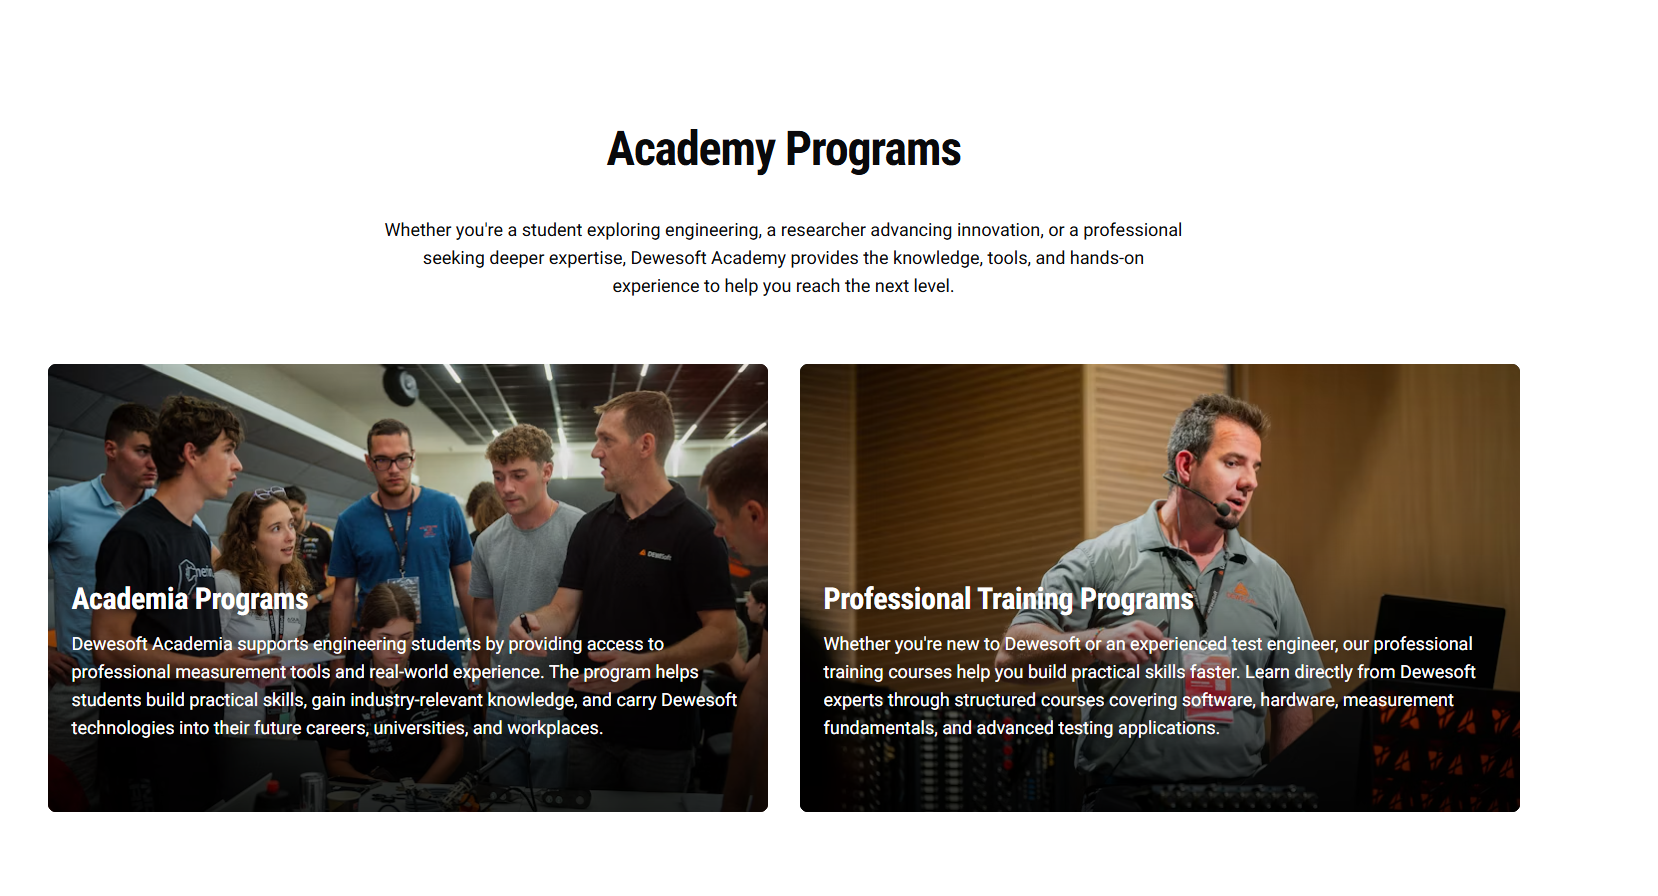
\includegraphics[width=0.8\textwidth]{dewesoft.png}
  \caption{Dewesoft Academy: programi (vir: \cite{dws-academy}).}
\end{figure}

\section{HBK Academy}
\subsection*{Opis}
HBK (Hottinger Brüel \& Kjær) je tekmec na področju merilne tehnike. Njegov HBK Academy ponuja seminarje in usposabljanja za strojno in programsko opremo~\cite{hbk-academy}.

\subsection*{Ključne funkcionalnosti}
\begin{itemize}
  \item katalog tečajev z opisom, trajanjem, lokacijo, jezikom in ceno; npr. enodnevni tečaj DAQ za 747~EUR~\cite{hbk-course},
  \item spletno usposabljanje v živo z aplikacijskimi inženirji~\cite{hbk-online},
  \item prenosi programske opreme, vdelane programske opreme (firmware) in priročnikov~\cite{hbk-downloads},
  \item pogodba o vzdrževanju programske opreme in podpori, ki vključuje popust pri tečajih~\cite{hbk-support}.
\end{itemize}

\subsection*{Prednosti in slabosti}
Prednosti: pregleden katalog tečajev s ceno in podatki o izvedbi ter strokovna podpora.
Slabosti: tečaji so plačljivi, termini pogosto »na zahtevo«~\cite{hbk-course}, napredna podpora pa je vezana na pogodbo~\cite{hbk-support}.

\begin{figure}[H]
  \centering
  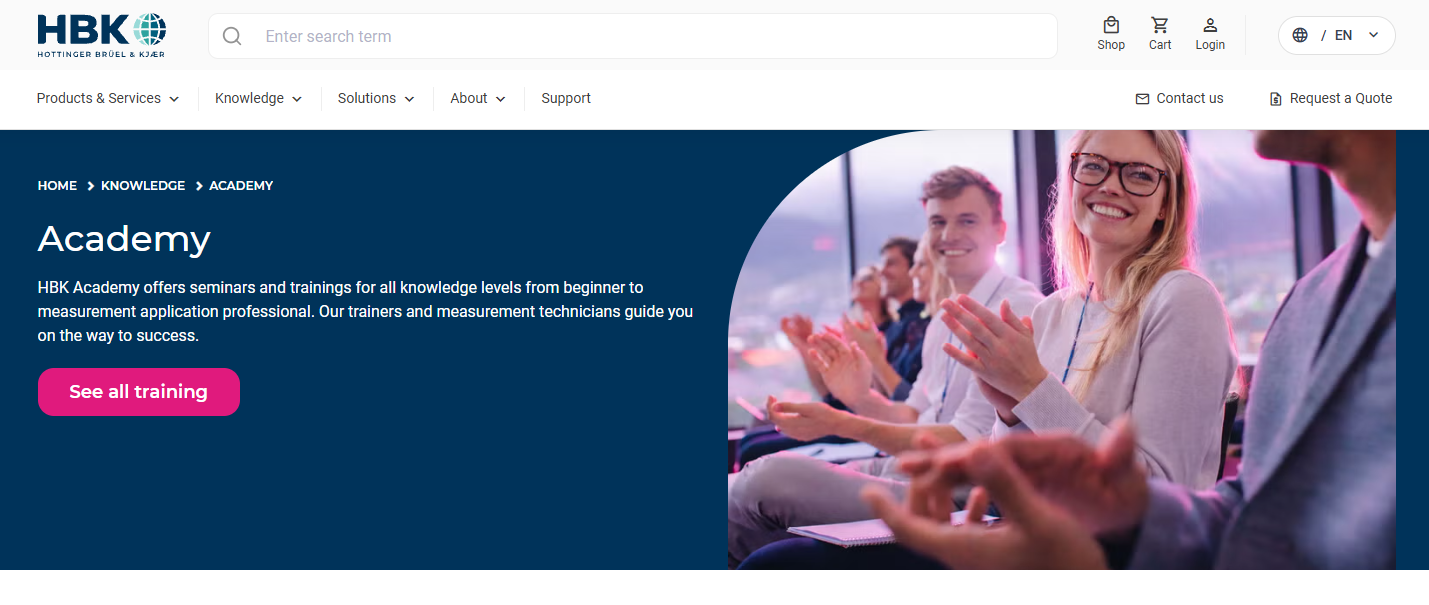
\includegraphics[width=0.8\textwidth]{hbk.png}
  \caption{HBK Academy (vir: \cite{hbk-academy}).}
\end{figure}

\section{NI (Emerson)}
\subsection*{Opis}
Podjetje NI ponuja spletišče z uporabniškim računom, ki združuje naročila, izdelke, podporo in učenje na enem mestu~\cite{ni-myni}.

\subsection*{Ključne funkcionalnosti}
\begin{itemize}
  \item moj račun: pregled naročil, ponudb in shranjenih konfiguracij, aktivacija izdelkov in prenos programske opreme~\cite{ni-myni},
  \item učni center z nadzorno ploščo učenca, vodenimi tečaji in spletnimi seminarji~\cite{ni-myni},
  \item podpora: dokumentacija, baza znanja, primeri kode, forum in oddaja zahtevka za servis~\cite{ni-dashboard,ni-search},
  \item obrazec za pomoč pri iskanju izdelka, ponudbi ali naročilu~\cite{ni-learn}.
\end{itemize}

\subsection*{Prednosti in slabosti}
Prednosti: vse kar stranka potrebuje (izdelki, ponudbe, podpora, učenje) je povezano z enim računom.
Slabosti: spletišče je zelo obsežno z veliko menijev, za servis in popravila pa je lahko potrebna veljavna pogodba o storitvah~\cite{ni-tutorials}.

\begin{figure}[H]
  \centering
  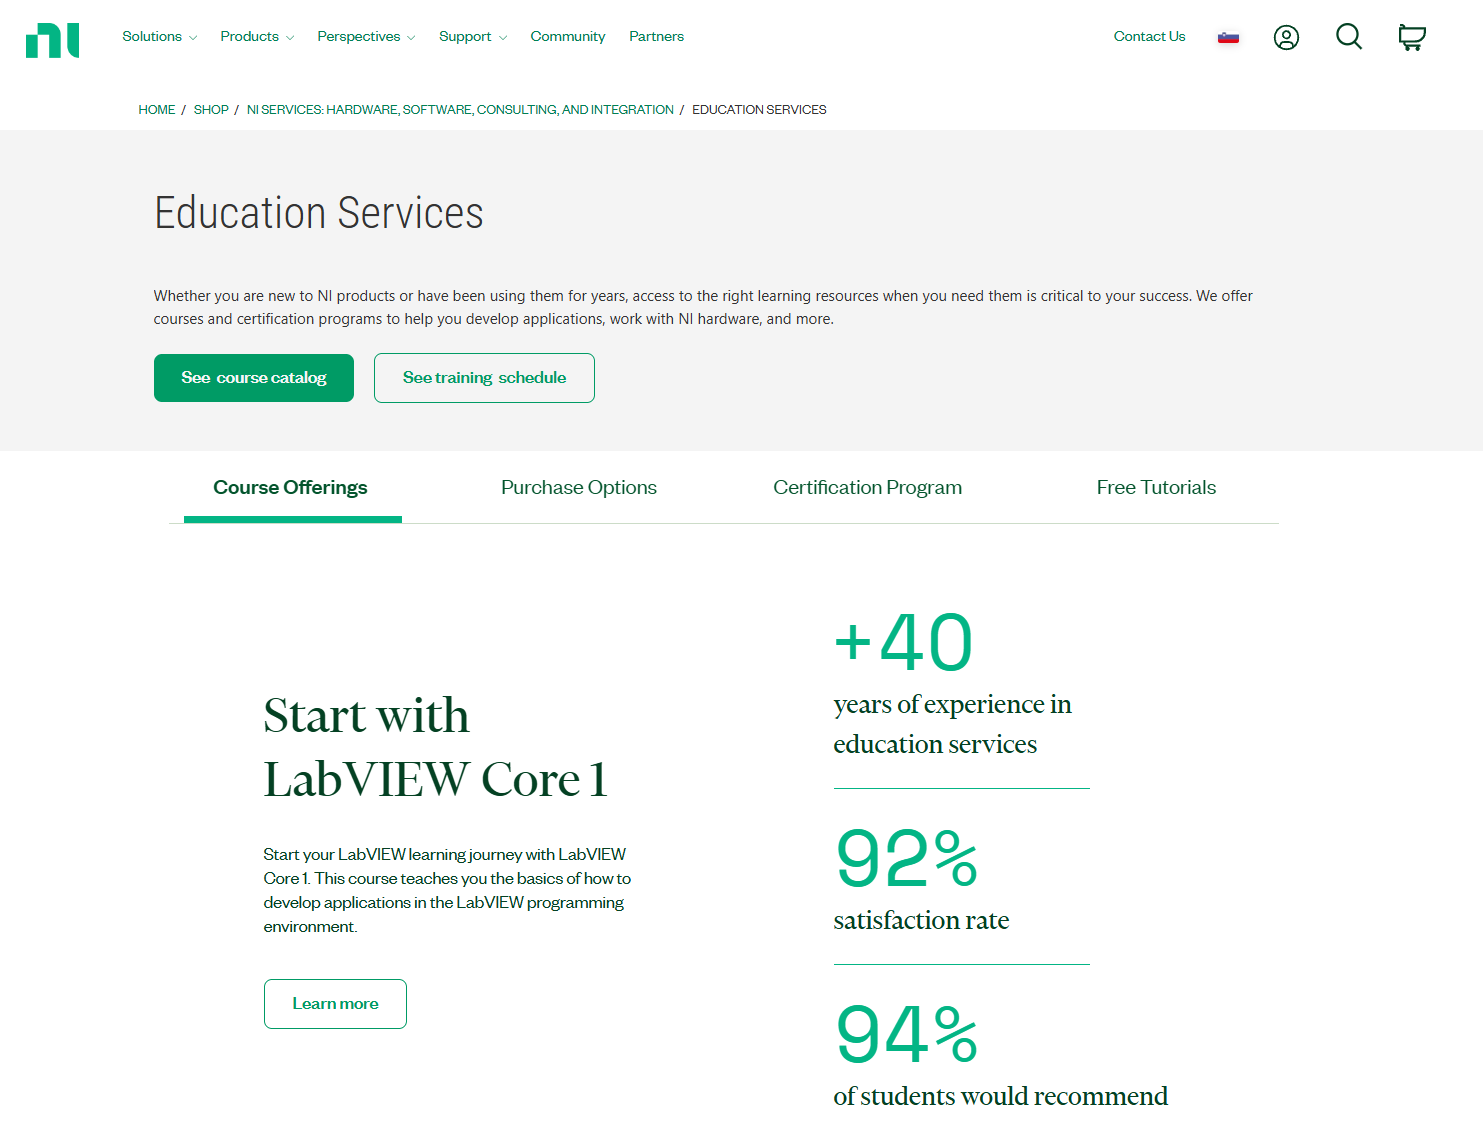
\includegraphics[width=0.8\textwidth]{ni.png}
  \caption{NI: Education Services (vir: ni.com).}
\end{figure}

\section{Zaključek}
\textbf{Kaj bomo prevzeli.} Od Dewesofta brezplačne tečaje in sistem napredka z zvezdicami, od HBK pregleden katalog z jasnimi podatki o izvedbi, od NI pa enoten uporabniški račun s pregledom izdelkov, podpore in učenja.

\textbf{Kaj bo drugače.} Naša rešitev združi izbiro opreme, podporo in izobraževanje v enem portalu za stranke Dewesofta, z enotnim iskanjem po bazi znanja, forumu in tečajih. Uporabniku predlaga tudi ustrezne tečaje glede na opremo, ki jo uporablja.

\begin{thebibliography}{99}
\bibitem{dws-signin} Dewesoft, \textit{Dewesoft Academy, podpora in baza znanja}, \url{https://dewesoft.com/signin}
\bibitem{dws-academy} Dewesoft, \textit{Dewesoft Academy}, \url{https://dewesoft.com/academy}
\bibitem{dws-online} Dewesoft, \textit{Dewesoft Online Training}, \url{https://dewesoft.com/academy/online}
\bibitem{dws-pro} Dewesoft, \textit{Dewesoft Online PRO training}, \url{https://training.dewesoft.com/online}
\bibitem{dws-prof} Dewesoft, \textit{Dewesoft Professional Training}, \url{https://dewesoft.com/academy/professional-training}
\bibitem{dws-academia} Dewesoft, \textit{Academic programs}, \url{https://dewesoft.com/academy/academia}
\bibitem{hbk-academy} HBK, \textit{HBK Academy}, \url{https://www.hbkworld.com/fr/knowledge/academy}
\bibitem{hbk-course} HBK Academy, \textit{Data Acquisition -- Selection of Parameters (ENC-DAT20H)}, \url{https://daqall-hbkacademy.talentlms.com/catalog/info/id:1942}
\bibitem{hbk-online} Brüel \& Kjær, \textit{Online Training}, \url{https://www.bksv.com/en/Training/online-training?sc_lang=en}
\bibitem{hbk-downloads} HBK, \textit{Downloads}, \url{https://www.hbkworld.com/en/services-support/support/support-bksv/downloads}
\bibitem{hbk-support} Brüel \& Kjær, \textit{Software Maintenance and Support Agreement}, \url{https://www.bksv.com/media/doc/bp1800.pdf}
\bibitem{ni-myni} NI, \textit{My NI}, \url{https://www.ni.com/myni/}
\bibitem{ni-dashboard} NI, \textit{My NI dashboard}, \url{https://www.ni.com/myni/dashboard/}
\bibitem{ni-search} NI, \textit{Support and discussion forums}, \url{https://www.ni.com/ja/search.html}
\bibitem{ni-learn} NI, \textit{Find the right product / Request a quote}, \url{https://learn.ni.com/courses/getting-started-with-veristand-2021-german}
\bibitem{ni-tutorials} NI, \textit{Request Support}, \url{https://www.ni.com/tutorials}
\end{thebibliography}
\end{document}